\documentclass[12pt]{article}
\usepackage[utf8]{inputenc}

\usepackage{algorithm}% http://ctan.org/pkg/algorithms
\usepackage{algpseudocode}% http://ctan.org/pkg/algorithmicx
\usepackage{graphicx}
\usepackage{fancyhdr}
\usepackage{setspace}
\usepackage{minted}
\usepackage{biblatex}
\usepackage{svg}
\usepackage{listings}
%inline verbatim%
\usepackage{fancyvrb}

\addbibresource{references.bib}

\pagestyle{fancy}

% remove header
\renewcommand{\headrulewidth}{0pt}
\fancyhead{}

% set margin
\usepackage[
  top=1in,
  bottom=1in,
  left=1.5in,
  right=1in
]{geometry} 

\begin{document}
\begin{titlepage}
   \begin{center}
        Kalamazoo College\\
        Senior Individualized Project in Computer Science
       \vspace*{3cm}
 
       \textbf{Developing a Reusable Framework for Data Fetching and Mutation}
 
       \vspace{0.5cm}
       GraphQL to SQL query mapping using existing Typescript technologies
 
       \vspace{1.5cm}
 
       \textbf{Joshua Gibson}
 
       \vspace{4cm}
 
       Faculty Supervisor:\\
       Dr. Eric Barth\\
       Assistant Provost and Professor of Mathematics\\
       Kalamazoo College\\
       Kalamazoo, MI
       
       \vspace{3cm}
       
       A paper submitted in partial fulfillment of the requirements for the degree of Bachelor of Arts at Kalamazoo College
       
       \vspace{2cm}
       2019
 
   \end{center}
\end{titlepage}

\pagenumbering{gobble}

%empty page
\null \newpage


\pagenumbering{roman}
\setcounter{page}{2}

\doublespacing

\addcontentsline{toc}{section}{Acknowledgements}
\section*{Acknowledgements}
This project would not have been possible without the help of dozens of people, both during the process of the SIP and before it was even a thought.  While this is by no means an exhaustive list, there are a number of people who must be thanked by name for their help.  I of course have to start by thanking my advisor Dr. Eric Barth for taking me on as an advisee.  This project has morphed a lot since he agreed to advise me on it, but he has been fully supportive in letting the project evolve naturally.  His guidance and support through these changes has been crucial.  In helping plan my initial project for my SIP, I must also thank Professor Andrew Koehler for his similar willingness to advise a project somewhat outside of his comfort zone.

As I developed the technologies discussed in my SIP over the summer, I would not have been able to do so without the mentorship and guidance of my co-workers at Maestro.  A huge thanks goes out to John Pinkster, Ben Meden, and Tyler VanderMaas for teaching me so much about back-end development.  Additionally, I have to thank Baxter Banghart for not entertaining phone calls throughout the summer where I would excitedly plan and develop these crazy ideas about GraphQL, but also for helping push me to be a better over the last eight years we've collaborated together.

This paper itself would also not be possible without the help of many people.  Thanks to Dr. Alyce Brady for entertaining my questions throughout the SIP Seminar and offering her years of wisdom she's gained through advising CS SIPs.  Thanks to all of my fellow CS students who proofread my paper as it was in the process of being written.  Additionally, thanks to my sister Amanda Gibson, for proofreading the paper as it neared its final draft.

Finally, I have to thank those who helped me get to where I am today.  A huge thanks goes out to Dr. Kelly Schultz.  She was the teacher who inspired my passion for Computer Science at such a young age and lead me to the computer science department at Kalamazoo College.  It makes me happy to know she's still teaching and inspiring young students today.  My other CS educators at Kalamazoo College, Dr. Alyce Brady, Dr. Pam Cutter, and Dr. Gerry Howser, have also played a huge part in developing me a computer scientist.  Without their education, I would not have the skills or ambition to tackle this kind of project.   And of course, I must also thank my parents, Scott and Kristine Gibson.  They have been nothing but supportive throughout all my education, whether it was helping me dual enroll in classes to help fuel my passion for computer science, encouraging me to study music in many different contexts and venues, or supporting me throughout college. No aspect of this project would be possible without them.
\newpage
\newpage

\section*{Abstract}
\addcontentsline{toc}{section}{Abstract}
This project seeks to develop a framework to minimize the amount of code required from developers to enable data fetching and mutation on a relational database.  Instead of manually generating SQL queries to interact with the database, GraphQL queries are translated to SQL by the framework.  Using technologies such as GraphQL, SQL, Nest.js, and TypeGraphQL, a set of reusable classes and functions are proposed that should ultimately reduce the amount of repetitive code in APIs developed for web-enabled applications. This project was developed within the context of a personal project, Practice Liszt, and throughout an internship and part time position at Maestro LLC in Kalamazoo, Michigan.  The framework proposed by the project is limited in its current GraphQL parsing ability but shows strong potential to integrate with these existing technologies to enable developers to extend the base creating, reading, updating, and deleting functionality.  In addition to the future improvements in GraphQL parsing in this project, other future framework features such as sorting, pagination, and filtering are discussed.
\newpage
\singlespacing
\tableofcontents
\doublespacing
\newpage

\listoffigures
\newpage


\pagenumbering{arabic}
\section{Introduction}

Programming is often a balance of writing original functionality while abstracting away often repeated code.  Instead of copying and pasting complicated code everywhere it is needed, developers seek to extract that code into its own function and reuse it through a project. This balance is a delicate game.  If the developer is left with less abstraction, they may have more control over their implementation. This lack of abstraction makes implementing new features difficult since every bit of functionality has to be re-written for each new context.  On the other hand, too much abstraction leaves the developer with little ability to adapt to their specific situation.

For small agencies that are contracted to create custom software, such as Maestro in Kalamazoo, MI, many common tasks are repeated:  services should have some form of authentication/authorization, keep track of users as they perform actions on a data set, and offer some way to request data from the service, among numerous other tasks.  While organizations over time build expertise in managing these aspects of systems, regardless of the skill of the developer, continually recreating each one of these subsystems takes a significant amount of time.  The question then becomes, what parts of this functionality could be reused across projects and what custom features should stay in individual applications.

This debate ultimately leads to what developers refer to as opinionated vs unopinionated frameworks.  An opinionated framework gives extra tools to reduce the amount of code that has to be written from scratch; however, there are often only a few correct ways to implement these features.  An unopinionated framework, on the other hand, gives the developer the basic tools needed to build their software, but the specific solutions they employ are often left up to the developer using the framework.

When I started working at Maestro as an intern and eventually Apprentice Software Engineer, the team I was a part of did have a standard way to build web servers, but they did not have framework in code to enforce those standards.  Each project was implemented in a very similar way, but features were still duplicated across each application.  For this reason, we have started to plan an opinionated framework that is specific to our team and would abstract away this repeated code.

As these framework conversations were beginning to develop, I also became interested in how to automate the translation of GraphQL queries into SQL queries.  These two languages, which are discussed below, are two common languages used to request data from a remote service.  GraphQL is focused on the communication between web browsers and web servers, whereas SQL is a language for requesting data from relational databases.  This translation functionality would allow web clients to request data from a server in any shape they desired.  Instead of the web server having to define queries for each shape of data needed by the client, the server could just respond dynamically to any data requested.  As I continued to investigate this feature, the applicability to an opinionated framework became clear.

In this paper, I will go into depth on my attempts to create a framework to automate the data fetching functionality of a web server. This framework will make it simple for a developer to define data types to be available in their web server and have those data types immediately available for clients to read, write, and update.  With this baseline functionality, duplicated code related to these operations can be removed from the software and will enable developers to maintain less code and develop more features.  This logic, however, is not specific to any project.  As will be discussed, the idea for this framework began in an independent project, was inspired by a project for Maestro, and has now developed into a project of its own.  The generality of this framework should allow it to be used for any application that needs a web server that exposes data from a database.

\section{Technologies}
Due to the varied background of those who tend to read senior individualized projects, this section seeks to introduce many of the technologies used and referenced throughout this paper.  Should the reader feel like they have a strong grasp on the following technologies, they may skip over these sections without missing content crucial to the rest of the paper.

\subsection{GraphQL}
The main technology motivating this project is GraphQL, a query language developed by Facebook in 2012 \cite{byronKeynoteBriefHistory2019}.  This language, in comparison to querying languages such as SQL (Structured Query Language), is designed to be exposed as to the web as a public set of defined functions.  Due to security concerns, SQL has been secured and users have been prevented from sending SQL queries directly to a database.  This allows GraphQL to be a public Application Program Interface (API), which is essentially a contract of what functions are available for a given piece of software.  GraphQL servers can define the available queries and mutations for the server, and the client is then only allowed to request those functions to be run by the server.

\subsubsection{Language Structure}

The unique aspect of GraphQL is that when the client requests data from the API, the client requests the shape of the response.  This means that rather than the server defining the exact data that it will provide, the client has the freedom to adapt the data requested.

Another unique part of the language is that data accessible by the API is represented as a graph of connected data types.  You could imagine each type of requestable data being a node on a graph where the edges represent relationships between the data.  When combining the ability to dynamically request data from the server and being able to request related data, the power of GraphQL becomes evident.  Since the client requests exactly what it wants and can receive all the related data in one request, the number of requests to the server is dramatically reduced and no extraneous data is sent to the client.

\begin{figure}[htbp]
    \centering
    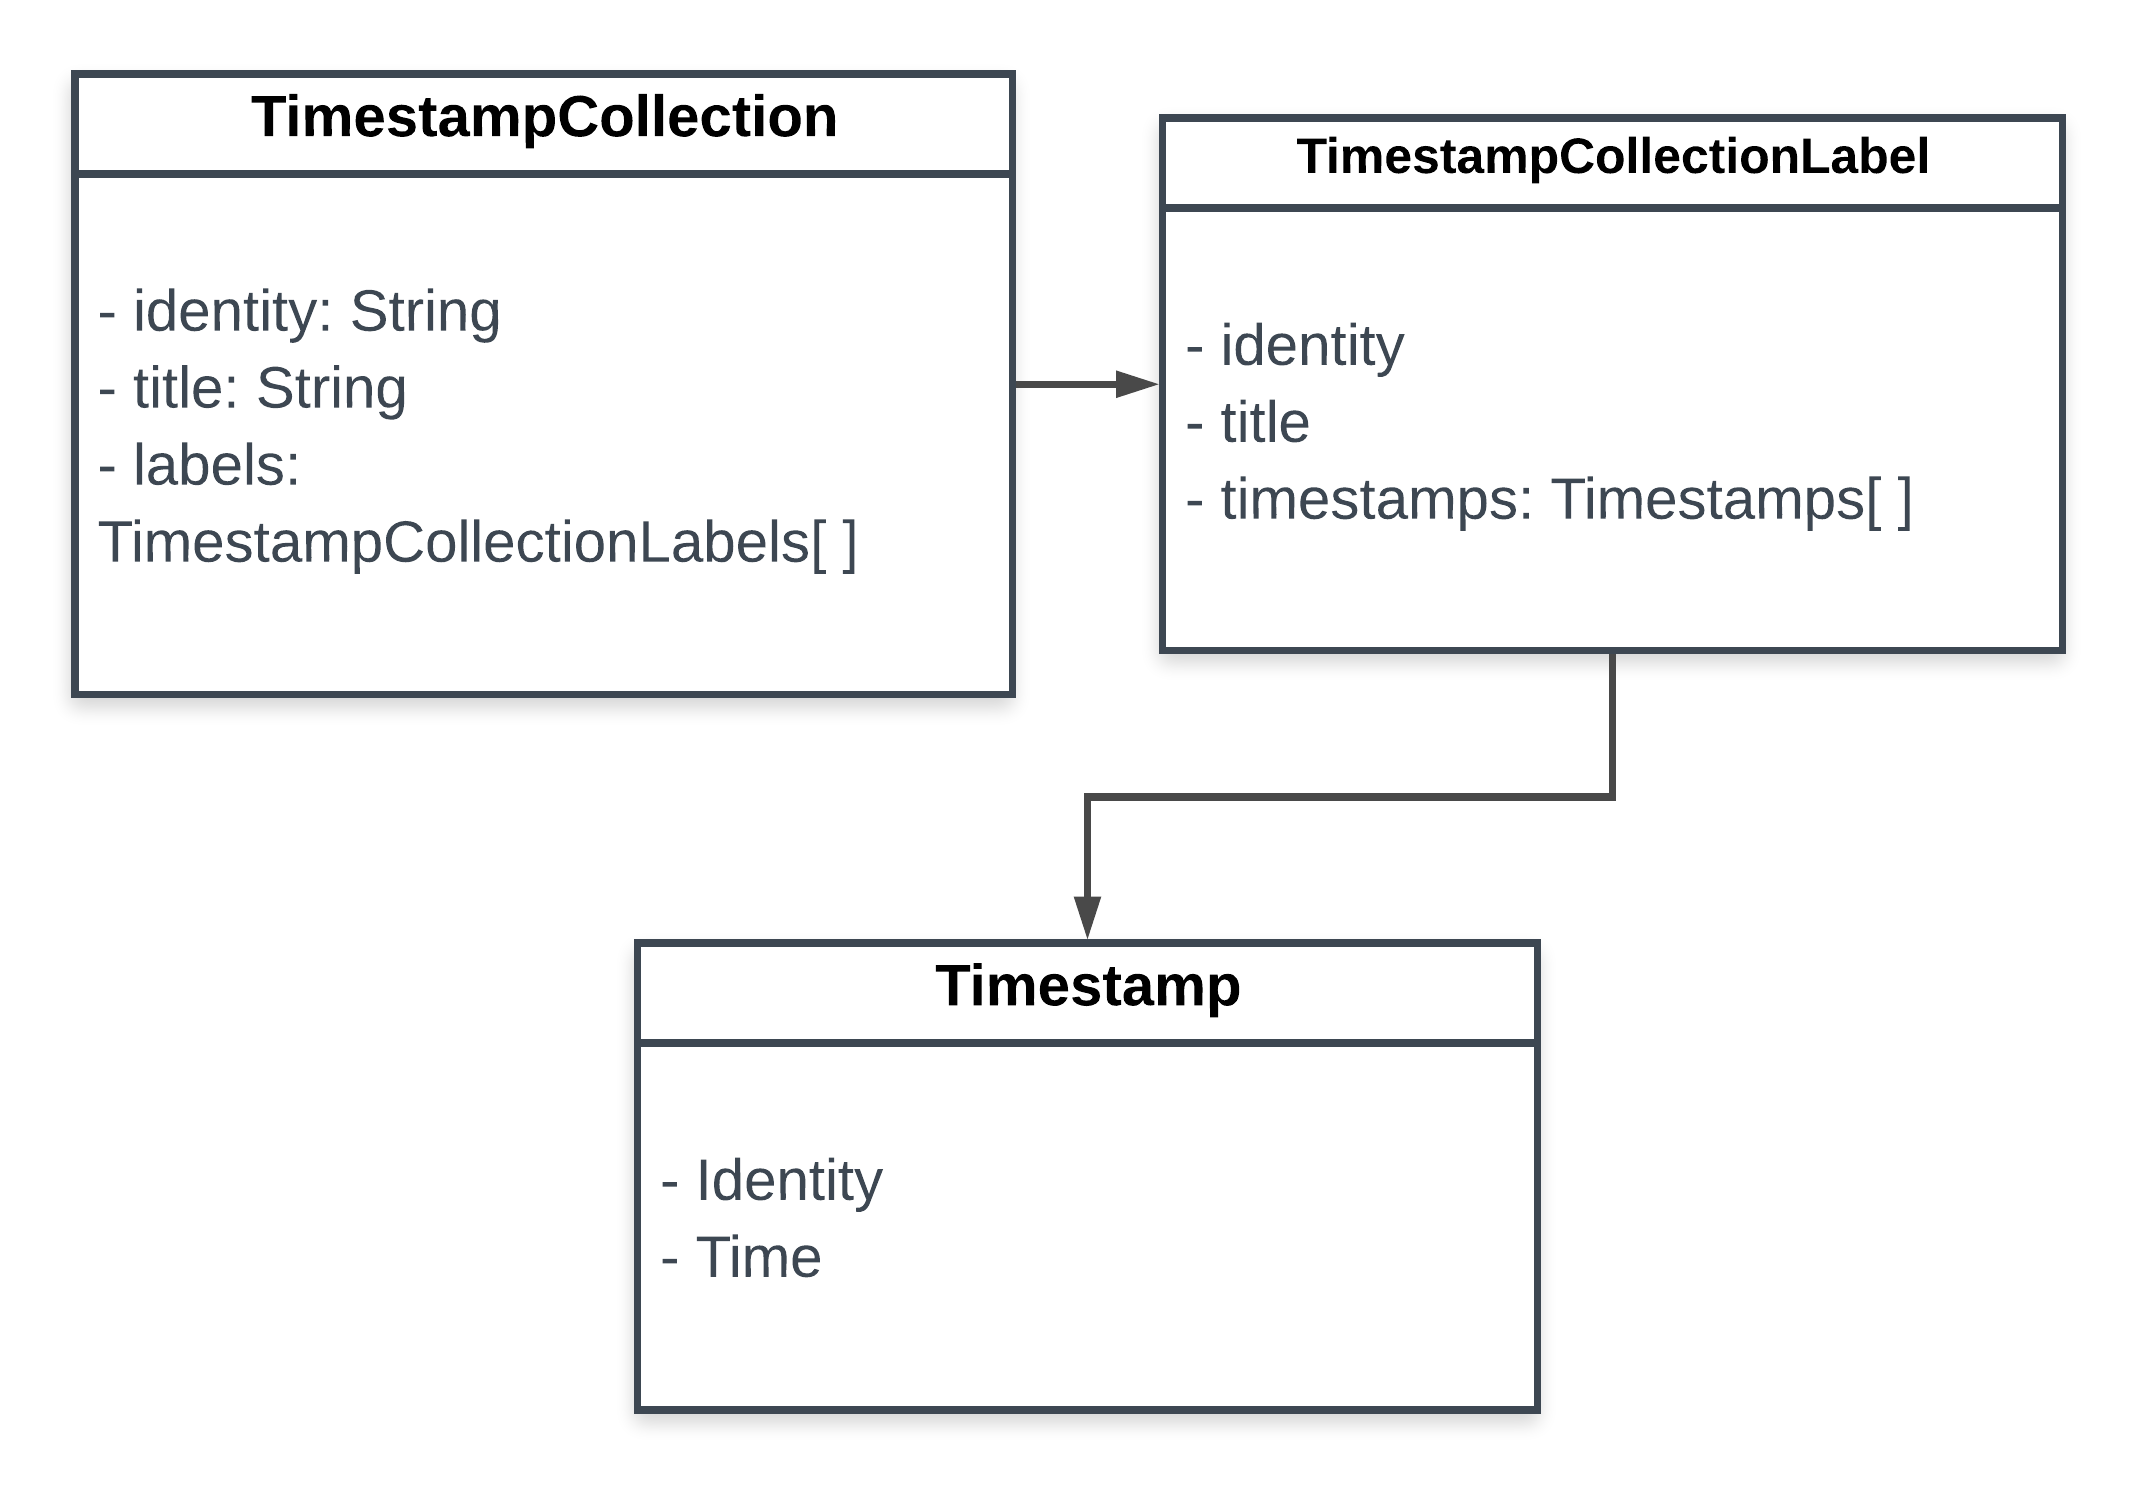
\includegraphics[scale=.15]{img/schema-graph.png}
    \caption{Visual representation of a sample GraphQL Schema}
    \label{fig:schema-graph}
\end{figure}

Figure \ref{fig:schema-graph} is a visual representation of a GraphQL schema with three types, TimestampCollection, TimestampCollectionLabel, and Timestamp.  The edges between each type show that relationships exist between the types. These relationships  would allow the user to create a request as shown in Figure \ref{fig:basic-query}.  The result of this query would be all TimestampCollections with their associated labels and timestamps.  If some of those requests fields or connected data not are needed, however, any part of that query could be removed and the API would respond with less data.

\begin{figure}
    \begin{verbatim}
query {
    timestampCollections {
        identity
        title
        labels {
            title
            timestamps {
                time
            }
        }
    }
}
    \end{verbatim}
    \caption{A basic GraphQL query}
    \label{fig:basic-query}
\end{figure}

\subsubsection{GraphQL vs. SQL}

SQL is debatably one of the most popular querying languages thanks to the popularity of relational databases, which will be discussed more below.  While the aim of this project is to connect GraphQL and SQL queries, it should be noted that the two languages exist for very different reasons.

SQL is a language very strongly tied to the storage and retrieval of data.  Queries act on specific tables that have strictly defined and structured data.  The SQL language does not make sense outside of the context of a relational database.  GraphQL on the other hand is completely agnostic to how the data is stored/retrieved.  The data source could be a relational database, a non-relational database, some other API, or could be programmatically generated. To fetch and update all of this data, GraphQL servers implement functions called resolvers that "resolve" the requested information from a data source.  That data source may be a  database, some other function in the code base, or calling another remote service..  Because of this flexibility, it is possible to use GraphQL as the query language for the front end of the application, such as the web browser or the user software, and SQL as the query language used by a GraphQL server to fetch or update data in a database.
\subsection{REST API}
In 2000, Roy Fielding wrote a PhD thesis focusing on the software architecture of web applications \cite{fieldingArchitecturalStylesDesign2000}.  In this dissertation, Fielding defined a style of designing web servers called Representational State Transfer (REST).  Since then, REST APIs have been the de facto standard for organizing services that send data over the internet.  Whether it is requesting individual web pages or bits of data to be used in an application, REST design patterns are often used. 

To this day, the basic constraints laid out in Fielding's dissertation are still used as the tenants of well designed RESTful interfaces.  A quick google search of REST principles will bring up hundreds of blog posts and tutorials summarizing these guidelines. For more information about REST, the reader is encouraged to do this additional research, however, I will include a brief summary below of the basic rest principles.

\subsubsection{REST Principles}

\begin{itemize}
    \item \textbf{Client-Server:} There should be a division between the software that stores and retrieves data and the software that displays the data.
    \item \textbf{Stateless:} All of the data required to respond to the request should be contained in the request. The server should not store the state of its interaction with the client. That is the client's responsibility.
    \item \textbf{Cache:} The results of a server request should be labeled as cacheable or non-cacheable.  Cacheable requests should not be re-requested for a certain time period to improve network efficiency.
    \item \textbf{Uniform Interface:} All REST services should respond in a uniform way, with each resource having a Unique Resource Identifier (URI).  Through these standard interfaces, web browser can go to nearly any web page without specific configuration.
    \item \textbf{Layered System:} The client is only aware of the top most layer of a REST system, but there may be many layers beneath the public facing layer that process the request.
    \item \textbf{Code-On-Demand:} The client can request code that extends the functionality of the application.  This is the basis of how browsers work.  They request code in the form of HTML, CSS, and JavaScript, which run on the machine and also often continue to request more code.
\end{itemize}

Thankfully, most of these principles are handled without much interference by the modern day developer. Caching, Layered Systems, and Code-On-Demand, are all key aspects implemented by web browsers and operating systems.  What takes most of the work on the developer's part is the organization of data into a Uniform Interface. In a REST API, if I want to request the TimestampCollection with an id of 1, the URI I use to request that resource might be \Verb"/api/timestampCollections/1".  Often, I would retrieve that information using an HTTP GET request.  An edit to that resource might then come through a PUT or DELETE request.

\subsubsection{REST vs. GraphQL}
For how often GraphQL is talked about as an alternative to REST APIs, it should be noted that many of REST's principles are typically implemented in a GraphQL API.  GraphQL servers respond to requests from client programs, GraphQL requests are often cached by their clients, such as the Apollo GraphQL client, and the web servers that respond to GraphQL requests are stateless and behind layered systems.  The biggest deviations from REST are in the fact that the organization of a GraphQL API is not through a Uniform Interface. In GraphQL all allowed queries and mutations are sent through a single `/graphql` endpoint.  Those requests then have a query name or mutation name attached to them that the GraphQL server interprets and knows how to respond to the client.  This allows for a much more flexible, but necessarily uniform, interface; however, since all requests are still over HTTP, a simple JavaScript client can allow almost any web page to interact with a GraphQL server.
\subsection{Modern JavaScript}

The original version of JavaScript was created in 1995 for the Netscape 2.0 browser and was prototyped in only ten days by Brendan Eich \cite{redhatinc.CreatingJavaScript}.  An article published in December of that year claimed that the new language designed for beginner programmers would make it easy for developers to interact with HTML and create web applications \cite{bucholtzNewLanguageAims1995}.  The language has since evolved greatly from that initial design.  The syntax has expanded, new environments for running JavaScript, known as run-times, have become standard, and whole variants of the language have been released and skyrocketed in popularity.  In this section, I aim to cover a few of the general developments in JavaScript as well as describe specific technologies that are utilized in my project.

\subsubsection{Node.js}
When designing applications that run on servers and machines, instead of in browsers, JavaScript, for many years, would have been seen as an unconventional choice.  Fourteen years after JavaScript's initial release, the release of Node.js changed this paradigm as it allowed running JavaScript outside of browsers. When the Google Chrome Project released its significantly improved V8 run-time for JavaScript, the engine was adapted into a server-side execution environment for JavaScript \cite{pramodEpisodeInterviewRyan}.  In an interview on the podcast "Mapping the Journey," Ryan Dahl, the creator of Node.js, claimed that he saw the asynchronous aspects of JavaScript, and the fact that it ran on a single thread, as making the language a perfect candidate for a robust, scalable, server-side language.  By simply adapting the browser's JavaScript engine to run locally on a machine, he unleashed JavaScript to the server environment.

Since then, Node.js and JavaScript have continued to grow in popularity. In last year's Stack Overflow developer survey, JavaScript was the most commonly used programming language and Node.js was the largest non-web/non-browser framework \cite{stackoverflowStackOverflowDeveloper}.

When discussing Node.js, the most important thing to understand is that it is simply a run-time to execute JavaScript on a machine without using a browser.  In practice, it has enabled JavaScript to become a first-class scripting language with full access to file systems, compiled libraries, and a dedicated developer community.

\subsubsection{TypeScript} \label{sec:typescript}
While Node.js adapted JavaScript for the server environment, a few years later, another technology, TypeScript, was created to adapt JavaScript to solve a different issue: static typing.  In its pure form, JavaScript is not a typed language, meaning that variables have no types, such as integers, strings, etc.  The variables are instead dynamic in type, which allows for great flexibility.  As Microsoft began working on web applications and started talking with their customers, however, they realized that JavaScript's lack of typings made managing large applications difficult.  One can imagine that as a code base grows, if there is no compilation step, small adjustments to the shape or type of data stored in variables or functions could be hard to catch.  With errors only surfacing at run-time, these applications became tough to maintain.  Microsoft's solution to this was to create TypeScript, a statically typed JavaScript variant \cite{idgnewsservicestaffMicrosoftAugmentsJavaScript2012}.

When writing in TypeScript, the syntax is nearly identical to JavaScript except variable declarations and function definitions also include types.  Before running a TypeScript program, this code is run through a compiler to ensure that all code is correctly using these typed objects. What makes TypeScript somewhat irregular amongst typed languages is that these types are completely removed at compilation time. The advantage to this is that TypeScript and JavaScript code are fully compatible.  Any TypeScript developer can thus take advantage of existing JavaScript libraries, and JavaScript developers are not required to adopt TypeScript to use these recently developed libraries.  As the developer writes their code, however, these types still exist, so IDEs and text editors can take advantage of the existing types to perform auto completion and check types inline.

Along with typings, TypeScript has also made other syntactic improvements over pure JavaScript.  The core feature utilized by this project has been the decorator syntax.  Introduced in version 1.5 of the language, TypeScript included this syntax while the feature was still in the proposal stage for future JavaScript support \cite{turnerAnnouncingTypeScript2015}.

In programming languages, reflection is the ability for a program to analyze and modify itself during run-time \cite{malenfantTutorialBehavioralReflection1996}.  In TypeScript, one of the common forms of reflection is using decorators to attach metadata to classes, properties, methods, and parameters.  By using a package called \Verb!'reflect-metadata'!, the program can reflect on itself to process the attached metadata and modify its behavior.  To illustrate this idea, I will introduce the server framework used in this project, Nest.js, which heavily relies on the use of decorators.

\subsection{Nest.js} \label{sec:nest-js}
Nest.js is a framework for creating server-side applications in JavaScript or TypeScript.  Along with Angular, the front-end framework that has heavily influenced Nest.js's design, the framework is object-oriented and uses metadata and decorators to declare the structure of the web server.

For example, imagine a simple web server that just responds to one HTTP GET request with a success message.  To define this endpoint, in Nest.js, the program must simply define a Controller, a class that responds to a number of HTTP requests, and a specific method to handle that request.

\begin{figure}
    \begin{verbatim}
import { Controller, Get } from '@nestjs/common';

@Controller('/api')
export class AppController {

    @Get()
    async respondToGetRequest() {
       return {success: true};
    }
}
    \end{verbatim}
    \caption{A simple Nest.js Controller}
    \label{fig:nest-controller}
\end{figure}

In Figure \ref{fig:nest-controller}, we see two examples of decorators: \Verb!@Controller! and \Verb!@Get!.  The former is what tells Nest.js that this class will have functions that respond to HTTP requests on the route \Verb!'/api'!.  The latter marks the function as the code that will return a response for a GET request on the route \Verb!'/api'!.  When these decorators are executed at run-time, they store metadata flagging the class as a controller and the function as an HTTP request method.  The Nest.js framework then reflects on the established metadata and routes the received HTTP requests to the appropriate functions.

As the framework has developed, numerous other features have been implemented and abstracted using decorators, such as request validation, authorization, and GraphQL definitions and resolving.

\section{Motivation}

\subsection{Practice Liszt}
My discoveries related to GraphQL began with a project I called Practice Liszt.  The main goal of the application was to be a rehearsal tool for musicians. As a percussionist, I found it difficult to practice along with video or audio excerpts on applications such as YouTube or Spotify.  As I would try to practice with sometimes 30 or 45 minute long videos, I would have to write down the times of different sections within a piece.  For example, if I wanted to start my practice at the beginning of as second movement of a piece, I would have to write down the time that occurs in the video, scrub to that time, and then start the video with enough time to pick up my instrument/implements and begin playing.

My intended vision for the project was to build a web application where one could create timestamps in these lengthy pieces of audio or video and keep them in an easily accessible list, hence the pun ``Practice Liszt.'' In the Spring of 2018, I did some basic research into the feasibility of this project.  I confirmed that the YouTube API had adequate controls to change the time of YouTube videos, that the interface could be easily created in React.js, a JavaScript UI Framework, and that GraphQL would be an appropriate means of communicating between the front-end (browser) of the application and the back-end (server and database) of the application.

After this initial mock-up, however, I did not work on the project again until the spring of 2019.  At the time I was interviewing for an intern position at the Kalamazoo company Maestro.  For my interview process, I had to implement a project that could show off my skills as a web developer.  Knowing I wanted to tackle this project in the future, I used this as an opportunity to create a complete prototype of the application.  By the end of the week, I had a working prototype that used React, GraphQL, and a non-relational database to store the timestamps called MongoDB.

Thankfully, the software team at Maestro was impressed by my project and I was offered an internship to work there. Going into the summer, I had planned on continuing to work on the project, from a feature standpoint, while I was not working at Maestro.  Ultimately, my goal was to have an application that was not only simple for a musician to use, but could also support use in academic research. On the musician side, they could create timestamps in multiple versions of a piece (think two different recordings, or a video and a piece of audio), and could set up privacy features which would allow them to either keep their timestamps private or share them with others.  For academics, I hoped that they would be able to look at what pieces have been timestamped and by extension, what recordings are associated with which pieces and what spots in the pieces are commonly timestamped.

To achieve this academic side of the project, I realized in July that I needed to redesign the data model.  In order to associate timestamps with actual published pieces of music, I decided to integrate my database with the MusicBrainz database, which is an open source database of music metadata, such as published works, composers, dates, and numerous other bits of data.  This database, however, was structured as a PostgreSQL database.  For this reason, my database went under a complete re-write between July and August to handle data retrieval from a relational SQL database instead of a non-relation database.  In the process of manually writing the resolvers which took GraphQL queries and responded with the appropriate data, I became frustrated with the need to manually define SQL queries that resolved a GraphQL query.  As I learned more at my internship with Maestro, I felt compelled to find a solution that would minimize the amount of work involved in mapping a GraphQL query to the data in a relational database.

\subsection{Maestro}
In June 2019, while working on my Practice Liszt project, I started working at Maestro. My main project over the summer was refactoring the back-end code for a learning management system called Loop.  Our goal  for the project was to move all of the existing code for the web server into the Nest.js framework (see Section \ref{sec:nest-js}).  In this process though, we used the refactor as an opportunity to remove a lot of duplicated logic throughout the code base.  Logic around data validation, processing HTTP requests, and permissions/authorization were all redesigned within the project to be more standard and less repetitive.

At the end of the processes, however, a lot of logic was still duplicated throughout the entire application.  Since the application has been written to have static REST endpoints, for every endpoint, we have to define exactly what data should be returned and how to fetch that from the database. With over two hundred endpoints, this creates code that is often doing the same thing, just in slightly different ways.  Moreover, whenever the front end of the application needs different data, a back-end developer has to make a change to the code to manually change or reformat the returned data.

As a developer at Maestro, while I was working on this refactoring project, I was also given the opportunity to participate in bi-weekly ``Developer Days.''  Somewhat inspired by Google's 20\% time, every other Friday, developers were encouraged to use their work days to work on any kind of software projects they were interested in.  The goal of the day was not to contribute productively to current projects, but to allow developers to explore topics and technologies that they were interested in.

Through my summer as an intern, I spent a number of my Developer Days focused on this idea of automated GraphQL/SQL queries. While I approached this problem from the perspective of my Practice Liszt project, the applicability to work projects became clearer the longer I worked on refactoring the Loop web server.  As I continued to share my progress from Developer Days, my coworker's interest in the project continued to grow and discussions began to occur about how we could potentially integrate this into future projects.  At the time of writing, our hope is that this system could be our standard way of exposing data from a relational database.

\section{GraphQL Query Mapping}

\subsection{Schema/Data Model}

The first step to mapping GraphQL queries to SQL queries is to define a shared schema between the allowed objects that can be requested in GraphQL and the tables in the relational database.  If the GraphQL schema and the database schema are defined in the same way, then each table in database becomes a GraphQL type that a client can request.

The first major design question was how to define these schemas at the same time.  In the JoinMonster library, the data model is only declared for the GraphQL schema and then the developer defines a map from the GraphQL types to SQL Tables \cite{carlJoinMonster}.  This way, the application can join the two tables together and resolve related data.  On the other hand, in Hasura, the GraphQL schema and the database schema are one in the same.  As you define the table schema that Hasura will use to generate SQL tables, a GraphQL schema is generated alongside it \cite{hasurainc.HasuraGraphQLEngine}.

In my solution, similar to Hasura, the data model for the GraphQL schema and the database schema are declared at once, however, they are declared in code instead of in a web interface.  To do this, I am integrating two libraries together: \Verb!type-graphql! for the GraphQL schema and \Verb!sequelize! for the database schema.  Thanks to another package called \Verb!sequelize-typescript!, both of these libraries allow for defining the schema using TypeScript decorators (see Section \ref{sec:typescript}).  As a result, by decorating a single, class that defines the schema for the data, I am given a GraphQL schema that defines that data is available, and a schema that used to make requests to the database.

\begin{figure}
    \begin{verbatim}
@ObjectType()
@Table({
    tableName: 'timestamp_labels',
    underscored: true
})
export class TimestampLabel extends CreatedByEntity<TimestampLabel> {

    @ForeignKey(() => TimestampCollection)
    @Column({
        type: Sequelize.BIGINT,
        field: 'timestamp_collection_id'
    })
    timestampCollectionId: number;

    @Field()
    @Column({
        type: Sequelize.STRING,
        field: 'title',
        allowNull: true
    })
    title: string;

    @Field()
    @Column({
        type: Sequelize.INTEGER,
        field: 'position'
    })
    position: number;

    @Field(() => TimestampCollection)
    @BelongsTo(() => TimestampCollection)
    timestampCollection: TimestampCollection;
}
    \end{verbatim}
    \caption{An example GraphQL/Database Schema}
    \label{fig:example-entity}
\end{figure}

Figure \ref{fig:example-entity} is based on an example from a \Verb!type-graphql! example project and shows how simple it is to define the schema.  The decorator \Verb!@ObjectType()! establishes the class as a GraphQL object type and the \Verb!@Table()! decorator says which table this object type maps to in the database.  Within the class, each \Verb!@Field()! decorator marks the property as being accessible in the GraphQL schema and each \Verb!@Column()! maps the field to a specific column in the database.  The \Verb!@BelongsTo()! decorator is what defines the relationship between two ObjectTypes/Tables.  This metadata is what is eventually used to join the tables together.

\section{Framework}
With the ability to map queries from GraphQL to SQL, the process of fetching data is reusable throughout the whole application; however, the developer would still have set up a resolver each available type and manually call the constructs include function.  To simplify this process, I have created a \verb!BaseEntity!, \verb!BaseService!, and \verb!BaseResolver! that when used together automate the process of creating queries and mutations for a given data type, fetching the data from the database, and returning the data to the client.  Moreover, these classes are extensible to allow custom functionality and extension by the developer.

\subsection{Dependency Injection}
The framework is heavily influenced by dependency injection, the pattern coined by Martin Fowler and popularized by the Java Spring framework \cite{fowlerInversionControlContainers2004}, and the Adapter pattern outlined in the book \textit{Design Patterns: Elements of Reusable Object Oriented Software} by Gamma, et. al \cite{gammaDesignPatternsElements1995}.  These two patterns when combined allow independent implementations of creating, reading, updating, and deleting data to be developed for each data type, while a standard interface allows for basic code to be reused across each data type.

\subsubsection{Dependency Injection}
The Dependency Injection pattern is a way of providing dependencies to an instance of a class, rather than them being defined in the class itself \cite{fowlerInversionControlContainers2004}. A dependency in this situation can be many things.  It might be an external code library, a object created within the application, or even configuration options for the application.  Instead of hard-coding these in to the software, dependency injection encourages flexibility in swapping out dependencies where needed. What this allows is for behavior to change for specific actions implemented by the dependency, while the implementation of the parent class does not have to change.  In my framework, the clearest use of dependency injection occurs between the \verb!BaseResolver! and the \verb!BaseService!.  The resolver class may define any number of queries or mutations on an object to either create an object, read an object from a data source, update an object, or delete an object (these operations are commonly abbreviated as CRUD).  The implementation for each of these actions on the database, however, may be different for each object type.  These implementations live in the subclasses of the \verb!BaseService!.  For a specific object type, a service class will be defined that contains the logic to perform all CRUD operations and an instance of this class is then injected into the resolver for that type.  Thus the resolver doesn't depend on a specific implementation for each type of object; it receives an instance of the service that knows how to modify the object in the database and simply forwards the requests to the service instance.

\subsubsection{Adapter Pattern}
The \verb!BaseService!, which is what is injected into the \verb!BaseResolver!, is also an example of the Adapter Pattern.  This pattern from Gamma's \textit{Design Patterns} is when a class wraps another existing class to provide additional functionality.  As will be discussed in more detail below, the \verb!BaseService! and its extending classes, are what communicate with the database.  Sequelize, the tool used to create SQL queries, already provides this functionality; however, at a framework level, we want to add another layer on top of Sequelize.  The \verb!BaseService! provides many of the same functions that Sequelize does, but also adds functionality such as error handling and combining queries to remove duplicated options when those Sequelize functions are called.  To do this, the \verb!BaseService! has its own functions such as \verb!create!, \verb!update!, and \verb!findOne! that call those same functions in Sequelize directly, while adding logic around them.  It is this service that is then used throughout the rest of the application, not the Sequelize code directly.  In this way, the resolver can take advantage of new functionality that allows it to take use the \verb!ConstructIncludes! to resolve GraphQL queries automatically.


\subsection{BaseEntity}

To avoid duplicating logic around retrieving data out of the database, it is beneficial for all database entities to share a common structure.  When I began working at Maestro, I was introduced to this pattern through the software team's use of a parent class called \verb!BaseEntity!.  This data model includes fields such as \verb!id!, \verb!identity! (a Universally Unique Identifier or UUID, instead of an integer id), and \verb!createdAt!, \verb!updatedAt!, and \verb!deletedAt! timestamps.  Once this class has been established, all other data models in the application should extend this \verb!BaseEntity!.  This way, for any type of data in the database, it is possible to retrieve the records since they all have an id an identity. Futhermore, this generates consistent metadata regarding their creation, modification, and deletion. When creating a service that will handle these operation, this baseline knowledge about each record is crucial.

By taking a subclassing approach to the data model, duplicating logic around these duplicated fields can also be avoided.  Looking back to the code example in Appendix \ref{ex:tl-entity}, the code does not specify that a \verb!TimestampLabel! has an \verb!id!, \verb!identity!, etc. Those basic fields are inherited from \verb!CreatedByEntity! which extends \verb!BaseEntity!.  This leads to yet another benefit of subclassing: there can be multiple levels of inheritance. For example, for many tables in the database, the user that creates the record should be tracked as well.  Having a \verb!CreatedByEntity! that extends \verb!BaseEntity! means that the \verb!created_by_id!, \verb!updated_by_id!, and \verb!deleted_by_id! can be added to this one model and never duplicated again throughout the code base.  Other models that are created by a user simply extend the \verb!CreatedByEntity!, thus receiving all \verb!BaseEntity! and \verb!CreatedByEntity! fields.

\subsection{Base Service}
With a standard structure for the data model of each type of data being stored, we can also create a standard set of functions related to creating, reading, updating, or deleting these records.  Once the data model has been established, Sequelize, library used to define the data model, provides a set of functions that directly interact with the database such as \verb!findOne!, \verb!findAll!, \verb!create!, etc.  The \verb!BaseService! wraps these functions to provide additional functionality, as well as enforce certain opinions on how to interact with the data.

\subsubsection{Merge Options}
When making queries to the database with Sequelize, the client is allowed to pass in options to modify the behavior of the query.  For example the options shown in Figure \ref{fig:merge-options} are all examples that would either include data of related tables in the request (through an \verb!include! option) or will limit the data that is returned (through \verb!where! options).  Throughout the \verb!BaseService! class, it will be useful to merge together two different sets of options.  For example, the application may allow the user to search for a timestamp label by its name; however, the user should only have access to labels that they created.  To achieve this, on each call to the database, we can merge in the option \verb!{ where: {createdById: user.id}}! so all requests have that constraint.  Because options are a mix of objects, such as \verb!where! options, and arrays, such as the \verb!include!, the logic to merge these options becomes somewhat complicated.  The solution I came to, however, is to do a deep merge on object values and to iterate through \verb!include! options and either add distinct model to the array, or deep merge matching models.  A deep merge is where the keys and values at each level of an object are combined. On each level, if both objects have the same key, their values are merged as well.  On leafs of the tree, meaning individual values instead of nested objects, one object's value is chosen to have the overriding value, and its value is used in the final result.

For certain parts of the query options, however, this default behavior doesn't work.  For \verb!include! values, for example, the overriding array at the top level would always be the one used, since it wouldn't know how to merge the arrays. Arrays are seen as ``values'', so they wouldn't be merged, but simply overridden.  For the key \verb!includes!, a custom function is given that looks through the two arrays to be merged, and it matches up the objects in the array by their model type.  If there are  two objects have the same model, the same deep merge algorithm is called on those two objects.  Otherwise each included object is added to an array that contains all of the requested models between the two options.

On \verb!where! options, the two \verb!where! clauses are simply wrapped in an \verb!AND! operator.  This allows both constraints to be applied, but no merge has to be computed.

Figure \ref{fig:merge-options} gives an example of what the outcome of this function would be for two example options.

\begin{figure}
    \begin{Verbatim}[fontsize=\footnotesize]
const initialOptions = {
    include: [{
        model: RelatedModel
    }]
    where: {
        createdById: 10
    }
};

const optionsToBeMerged = {
    include: [{
        model: RelatedModel,
        include: [{
            model: ASecondModel
        }],
        where: {
            createdById: 10
        }
    }],
    where: {
        name: 'A Value'
    }
};

const optionsAfterMerge = {
    include: [{
        model: RelatedModel,
        include: [{
            model: ASecondModel
        }],
        where: {
            createdById: 10
        }
    }],
    where: {
        [Op.and]: 
        [
            {
                createdById: 10
            },
            {
                name: 'A Value'
            }
        ]
    }
}
    \end{Verbatim}
    \caption{Example Sequelize Options}
    \label{fig:merge-options}
\end{figure}

\subsubsection{Base Find Options}
With the ability to merge query options, the \verb!BaseService! provides a mechanism of not only overriding the standard behavior of requests on each method call, but it also provides the option to base level constraints on each query.  When extending the \verb!BaseService! class, the subclass can override a function called \verb!getBaseFindOptions!.  This function is called for every fetch to request data from the database and the options it returns are merged into options provided by caller.  A common use case for this would be to use this function to ensure that the user can only access records they created.  Looking at the example service in Appendix \ref{ex:tl-service}, we can see how crucial this ability to limit access is.  For Timestamp Labels, they should only be viewable by the user that created that label, or by any user if its collection is marked as public.  By defining a \verb!getBaseFindOptions! method on an implementing service, that logic is applied to all access operations on this object type.  

This is one of the largest benefits of this framework versus Hasura or JoinMonster.  Since functionality is kept in extendable classes, this kind of behavior can be modified for each type defined in the application. Additionally, because the data model defined in the entity is defined for a fully functional ORM, the developer can use that same data model to modify the functionality of their service. No re-definition has to occur.

\section{Query Mapping Limitations}
The main limitation on this project is that query mapping as it stands is incomplete. As implemented, the algorithm assumes that there is only one GraphQL request being made at a time.  In the GraphQL specification, and in Nest.js's implementation, multiple GraphQL requests can be sent at once and the server will respond once with the result of both queries.  If multiple queries are sent, the \verb!ConstructsInclude! function would return the includes options for the first query for all requested queries.

To adjust the \verb!ConstructIncludes!, instead of just inspecting the top level query, the function will instead analyze each query separately.  The major difficulty is that the caller will need to tell the \verb!ConstructIncludes! function which query should be analyzed. Typically, this would happen in the resolver class when it calls the \verb!ConstructIncludes! function. The first course of action would be to attempt to retrieve this information from Nest.js.  Somehow Nest.js knows which resolver functions to call based on the GraphQL queries it receives, so it must have some metadata stored about which query is being request by the client.  Once it is determined how to retrieve this information from Nest.js, the adjustment to the \verb!ConstructsIncludes! can be completed.

Additionally, the query mapping does not currently support union types.  These would occur if the server could return multiple different object types on a single connection.  The example in the GraphQL documentation for union types is a search that could return three different types.  The GraphQL request for that function would then specify what fields they want for each those types.  The problem with trying to support union types is that they do not fit well with relational databases.  In a relational database, it is known what the type of each related data is.  At the core database level, it is not possible to store a union type.  There is a way to simulate this flexibility which is known as polymorphic table design.  In this situation, you store a reference to the associated data and store another field denoting what type of data is in the referenced table.  This breaks the ability to have those references as foreign keys in the database, which is the main building block of relational databases. These tables can be useful, but ultimately present significant challenges to traditional relational database design.  For this reason, mapping GraphQL union types to a relational database becomes a complicated task.  As long as this project continues to focus on mapping GraphQL queries to SQL queries, this problem will likely not be a major focus.

Overall, the project works as I hoped it would, but it requires the user to limit their use of GraphQL.  Additionally, developers must be aware of these limitations.  If this project were open-sourced today and other developers began using the framework, it would likely be a frustrating experience discovering what features they could use and what they could not.  To address these issues, additional research into the GraphQL Abstract Syntax Tree and how to parse computer languages in general, will need to be conducted and documented.

\section{Future Work}

The majority of future work is centered around customizing the resolver.  When developing an application, it is common to need the ability to dynamically filter and change the data set being returned by a query.  For example you might want to change the order that data is returned, only want to view a page's worth of data, or only want to query objects where a certain condition is true or false.  Each one of these actions would be prompted by different parameters on the query.  In this section, I will propose how those features might look for the developer once they are fully implemented.

\subsection{Pagination}

A common feature of large applications is viewing paginated subsets of data.  For example, in the Practice Liszt app, there might be thousands of public timestamp collections, but the user can only view ten at a time on the displaying web page.  The GraphQL server then needs a way to deliver these thousands of records in pages of ten records at a time to the client.  I believe this feature will be possible to integrate into my framework, but will require effort in both research and implementation.  At the resolver level, the number of results per page and the page to retrieve will have to become arguments for each paginated query. These options will then be merged into the service's options so only that subset of data is retrieved from the database.  Additionally, a default sort order will have to be chosen before paginating the data.  If no default sort order is determined, the database doesn't know what order the ``pages'' are in.  If the order is left random, ``Page 2'' will be different every time.  By having a default sort order, as the client requests subsequent pages, only new data will be returned on each request.

\subsection{Sorting}

In addition to a default sort order, it will also be necessary to allow the client to modify the sort order of the results.  In a web application, it is common to change sorting from alphabetical by name, to reverse alphabetical, or sometimes a different property such as creation time.  The goal would be on the top level of the query, the client would be able to select an argument specified from a list of pre-defined sortable properties.

These sortable properties could be defined in two places.  Option one would be in the resolver.  This could become another option of the base resolver where the developer simply provides a list of sortable properties.  The resolver then provides those as possible arguments to the client.  A potentially more elegant, but more complicated, solution would be to have a decorator on the entity that marks those database fields sortable.  The resolver would then look at the entity and identify its sortable fields and use those for the list of acceptable sorting properties.

\subsection{Filtering}

The most complicated bit of key functionality left to implement is filtering data based on arguments passed to the query.  An example of this would be searching for a certain Timestamp Label.  On the query, you might provide it a string to match and only Timestamp Labels that match that key will be included in the data set.

The difficulty in this use case is determining where to define the filtering behavior and at what step in the process to actually inject the filter into the query.  Ideally, the definition of the filter will be on the resolver. At this level, the developer will declare what arguments are available to the the client and will also define what behavior the filter will have.  Applying the filter to the query will have to occur in the \verb!ConstructIncludes! function, however.  Since multiple filters could be applied at multiple levels of the query, it is not enough to just process the top level arguments.  The \verb!ConstructIncludes! function will need to parse the parameters at each level and determine what filters should be applied.  It will then inspect the metadata applied to the resolver to retrieve the defined behavior.  That behavior will be executed and then inserted into the query.  The parsing problem in this situation is similar to sorting, but since the behavior is far more dynamic than sorting, the implementation within that function will be much more complicated.

\section{Conclusion}

Designing a new framework for developing web application back-ends is no small tasks.  Open source communities of thousands of people support some of the largest frameworks that have taken years to develop. Throughout the paper I have used this idea of a framework to describe the three key reusable entities I have developed, \verb!BaseEntity!, \verb!BaseService!, and \verb!BaseResolver!.  What these classes should provide to the developer is a clear and opinionated way to structure their GraphQL servers.  Additionally, by using this base structure, some basic functionality surrounding reading and writing the data will also be available by default.

In contrast to most frameworks, however, this project relies heavily on on other projects, notably Nest.js, Type-GraphQL, Sequelize, and Sequelize Typescript.  Rather than trying to re-write these projects to work exactly as desired, the project augments each project in specific ways to work work together and speed up development time while reducing repeated code.

Looking back to the summer when this project developed, it was my frustration with the amount of repeated code that I found across my personal and work projects.  By providing a set a of base classes to use throughout an application, this framework has the potential to reduce duplicated code related to creating, reading, updating, and delete data from a database.  It is also flexible enough, to leave room for some custom implementation.  This is necessary since each app will be developed in its own context, but it also leaves room for misuse.  A developer could ignore the patterns provided by the three base classes and continue to duplicate logic throughout the application.  As is always the case will programming, clean and maintainable code will only come through a combination of design and discipline in implementation.

As we continue to refine are development process at Maestro, creating more re-usable patterns will be our goal moving forward.  Even across projects, we want to move to have one opinionated and pre-implemented way to do as much of our projects as possible.  This way, those apps that don't need custom functionality will no longer has to re-implement the same features over and over again.  This project simply focuses on data mutation and data retrieval using SQL and GraphQL, but so many other features could implemented in an opinionated and reusable way.  A code library with basic implementations for authentication, data retrieval, error handling, and many other features would enable us to develop applications for a clients at a speed we have not been able to achieve previously.
\newpage
\setcounter{page}{1}
\addcontentsline{toc}{section}{Appendicies}
\appendix
\section{Code Example: Timestamp Label}

\subsection{timestamp-label.entity.ts}\label{ex:tl-entity}

\lstinputlisting[
    basicstyle=\footnotesize,
    numbers=left
]{code/timestamp-label/timestamp-label.entity.ts}

\subsection{timestamp-label.service.ts}\label{ex:tl-service}

\lstinputlisting[
    basicstyle=\footnotesize,
    numbers=left
]{code/timestamp-label/timestamp-label.service.ts}

\subsection{timestamp-label.resolver.ts}\label{ex:tl-resolver}

\lstinputlisting[
    basicstyle=\footnotesize,
    numbers=left
]{code/timestamp-label/timestamp-label.resolver.ts}


\newpage
\printbibliography
\addcontentsline{toc}{section}{References}
%\bibliographystyle{plain}
%\bibliography{references}
\end{document}
